La presente memoria refleja el trabajo realizado por Javier Cejudo a lo largo
del proyecto que lleva como título ``\textit{Herramienta de apoyo para la
gestión de recursos humanos en el desarrollo de proyectos de I+D}". El
determinativo \textit{de apoyo} hace referencia a que la herramienta está
pensada para \textit{dejar hacer} y detectar los errores, en lugar de \textit{no
dejar hacer} y proponer soluciones. Esta característica, que define gran parte
de la filosofía de la aplicación, es un requerimiento del cliente, la empresa
Ingeniería e Innovación, en la que el proyectante estuvo haciendo prácticas de
empresa durante varios meses. De algún modo, podría decirse que la aplicación
funciona a modo de auditoría para asegurar que los datos que se manejan son
consistentes. La referencia a los proyectos de I+D indica que está orientado a
la forma en que los entes públicos gestionan la concesión de subvenciones a este
tipo de proyectos: presentación, aprobación y justificación del proyecto.

El proyecto comenzó como una de las labores del proyectante en la citada
empresa, y no se convirtió en su proyecto hasta pasados algunos meses, cuando
su tutor de empresa sugirió la posibilidad de que esa labor de diseño e
implementación constituyera su Proyecto Fin de Carrera. Puesto en
contacto con Ángel Luis Rubio García, tutor académico de las
prácticas que el proyectante desarrollaba, se llegó a la conclusión de que, en
efecto, el trabajo realizado hasta ese momento, y que seguiría durante algún
tiempo, se encontraba entre los límites de lo que debe ser un Proyecto Fin de
Carrera.

El principal inconveniente, y nada pequeño, es que el proyecto ya estaba en
marcha y no se había seguido la metodología típica en estos casos, a saber: no
se había desarrollado un Documento de Objetivos del Proyecto ni se había
elaborado un Plan de trabajo. En la primera reunión con el tutor académico, se
llegó a la conclusión de que, dadas las circunstancias y dado que la parte
técnica del proyecto ya estaba bastante avanzada, no debía realizarse un DOP ni
un plan de trabajo, pero sí debía tratar de documentarse con el mayor detalle
posible cuál había sido la carga real de trabajo y su distribución en el
tiempo. Esto fue posible debido a que, siguiendo la metodología de la empresa,
se llevó un registro diario de las actividades que realizaba cada estudiante en
prácticas.

\section{Antecedentes}
\label{sec:antecedentes}

Ingeniería e Innovación\footnote{Ver página web de la empresa:
\href{http://www.ingenieriaeinnovacion.com/}{
http://www.ingenieriaeinnovacion.com/}.} es una empresa cuyo principal
objetivo es ofrecer a las empresas servicios avanzados en gestión de la
innovación y de los procesos de I+D. Estos servicios van desde la presentación
de proyectos de I+D a programas regionales, nacionales y europeos de ayudas,
hasta la búsqueda de socios tecnológicos, pasando por búsqueda de patentes o la
obtención de seguridad jurídica a la hora de aplicar deducciones fiscales.

Las labores del proyectante en el seno de la empresa han sido diversas:
\begin{itemize}
\item recopilación de información de apoyo a los proyectos acerca de los campos
más diversos relacionados con la investigación de procesos innovadores;
\item redacción de proyectos circunscritos a las tecnologías de la información;
\item labores de apoyo administrativo;
\item reforma de la interfaz de usuario de la herramienta de gestión de la
empresa y
\item desarrollo web para la gestión de los recursos.
\end{itemize}
Fue de esta última actividad de la que surgió el proyecto que nos ocupa en esta
memoria.

Ingeniería e Innovación ya disponía de una Intranet para la gestión de algunos
de los datos que maneja: clientes, facturas, contratos... y los temas
que van a entrar en interacción directa con la herramienta desarrollada por el
proyectante: proyectos y expedientes. Estos últimos son cada una de las
propuestas de subvención realizadas para cada proyecto: por ejemplo, un mismo
proyecto puede tener dos expedientes diferenciados si se ha solicitado una
subvención tanto a la ADER con su convocatoria de Innovación y Desarrollo
Tecnológico como por los planes nacionales AVANZA para el desarrollo de la
Sociedad de la Información y del Conocimiento. Sin embargo, la información que
se guardaba hasta ahora se refería al estado de las propuestas, a las fechas
límite de entrega de las memorias de presentación o justificación, a quién era
el responsable del proyecto dentro de la empresa... En definitiva, nada
relacionado con la gestión de actividades o recursos implicados en el
desarrollo del proyecto.

\section{Motivación}

La motivación principal para la elección de este proyecto se basa en la propia
naturaleza del mismo: una aplicación web. A pesar de que hoy en día estamos muy
acostumbrados a las aplicaciones web con, por ejemplo, servicios de correo
electrónico que poco tienen que envidiar a sus homólogos de escritorio, todavía
está emergiendo la tendencia de ofrecer aplicaciones interactivas directamente
en nuestro navegador. El proyectante, sin embargo, tenía la sensación de no
haber explorado este campo con la suficiente profundidad a lo largo de sus
estudios académicos y encontró en el Proyecto Fin de Carrera la figura perfecta
para realizar una toma de contacto con tecnologías con las que tenía poca o
ninguna experiencia: PHP, JavaScript, Ajax, HTML DOM...

Asimismo, el proyectante encontró una gran motivación en el hecho de que se
tratase de un proyecto real con inmediata aplicación para la empresa. La
posibilidad de llevar a cabo un proyecto vinculado a una empresa recordó al
proyectante unas palabras de Julio Rubio acerca del éxito que suponía que más de
la mitad de los proyectos realizados hasta 2008 estuvieran vinculados a
empresas: «Hemos logrado salir del marco académico y hemos afrontado problemas
reales de las empresas» \footnote{Como se puede leer en la siguiente
dirección:\newline
\href{http://goo.gl/S0dIO}{http://www.larioja.com/20080423/rioja-region/...}} .


\section{Necesidad del proyecto}
\label{sec:necesidad}

La herramienta surge de la nueva necesidad de la empresa Ingeniería e Innovación
de tener un registro mensual de las actividades realizadas por los
empleados de sus empresas cliente implicados en la realización de los proyectos
de innovación presentados a convocatorias de la ADER (Agencia de Desarrollo
Económico de La Rioja), fuente de financiación de una buena parte de los
proyectos gestionados por la empresa. En resumen, donde antes solamente se
exigía un desglose anual en la etapa de justificación de los costes de recursos
humanos, se pasó a exigir un detalle mensual desglosado por las actividades
realizadas en el marco del proyecto.

El problema radicaba en la forma en que se gestionaban estos datos. Ingeniería e
Innovación llevaba un registro anual de las horas que cada empleado había
desarrollado o supuestamente iba a desarrollar en un año concreto, dependiendo
de si los proyectos a los que se referían esas horas estaban en fase de
presentación, aprobación o justificación. El soporte de tal registro no era sino
una hoja de cálculo como la de la figura \ref{fig:hoja_calculo}.

\begin{figure}
\centering
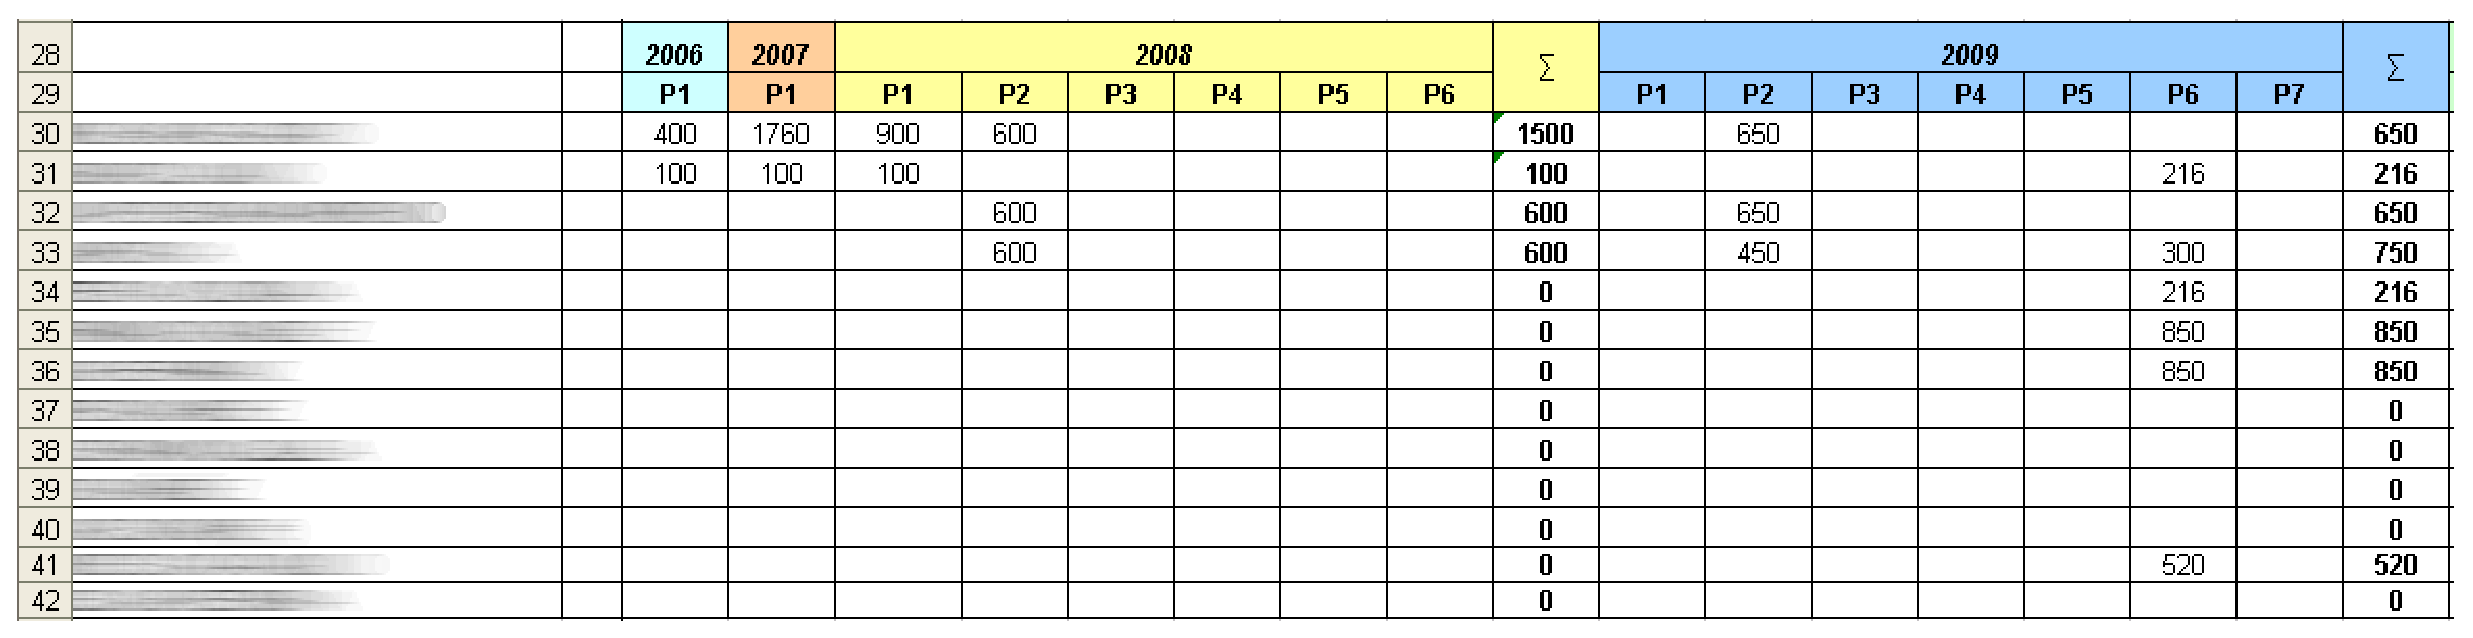
\epsfig{file=imagenes/registro.eps,width=5.28in}
\caption{Hoja de cálculo con el registro de horas asignadas.}
\label{fig:hoja_calculo}
\end{figure}

Por si no se aprecia adecuadamente en la imagen, las dos primeras columnas
coloreadas corresponden a un mismo proyecto en los años 2006 y 2007, y sólo
contienen datos de dos empleados. Las subdivisiones de la columna amarilla
corresponden a diversos proyectos cuyo desarrollo se extendía en el año 2008, y
de nuevo reflejan la carga de trabajo de cada empleado a lo largo del año
completo. Los datos son proporcionados por la empresa coordinadora del proyecto
y el objetivo de este registro no es otro que comprobar que no se están
imputando por error más horas a cada trabajador que las que tiene en su convenio
de trabajo. En este caso se está mostrando la tabla de horas justificadas, es
decir, horas que se llevaron a cabo una vez el proyecto estaba aprobado por los
organismos oficiales. Del mismo modo, existe una tabla para las horas
presentadas, ya que tampoco deberían proyectarse más horas de las que un
empleado puede llegar a trabajar.

Los problemas que se derivaban del uso de esta metodología eran diversos y de
difícil solución sin un rediseño completo de la metodología, a saber:
\begin{itemize}
\item la empresa cuenta con una base de datos de proyectos que no puede
contrastarse con la hoja de cálculo, de modo que debe comprobarse manualmente
el estado del proyecto para saber la naturaleza de las horas que deben ser
tenidas en cuenta;

\item no se guardaba registro de las horas del convenio colectivo, ni de la
fecha de alta o baja de los trabajadores, de manera que no podía asegurarse que
las horas imputadas no sobrepasaban las debidas;

\item el formato requería un alto grado de mantenimiento aun cuando no
contempla la nueva necesidad de especificar las horas por meses y actividades
individuales, en lugar de anualmente por proyectos. La nueva necesidad
simplemente era impracticable con el antiguo formato;

\item cualquier resumen de las horas asignadas que quisiera extraerse desde los
datos de la hoja de cálculo (por ejemplo: horas asignadas a un proyecto en
todos los años que abarca su desarrollo, horas asignadas a un empleado en
cualquiera de los proyectos en los que interviene...), debía elaborarse
manualmente por un trabajador cualificado, lo que consumía unos recursos que la
nueva herramienta reducirá al mínimo;

\item el antiguo formato tampoco guardaba registro del coste/hora de los
empleados, que varía, por lo general, anualmente, de modo que no se podía
calcular automáticamente el coste de los recursos humanos de los proyectos;

\item afinando un poco, es fácil deducir que no se puede llevar un registro de
proyectos en colaboración que, bien no duplique información ocasionando de nuevo
inconsistencias potenciales, bien no cause un aumento en el trabajo de
gestión: si tenemos varios clientes colaborando en un mismo proyecto debemos,
bien duplicar la información de los empleados para que figuren en las hojas de
cálculo de los otros clientes, bien consultar cada hoja de cálculo si
queremos extraer información acerca del proyecto en colaboración; 

\item a pesar de que podía detectarse cuándo se hizo la última modificación de
la hoja de cálculo, era imposible comprobar individualmente la actualidad de los
datos disponibles o quién los había modificado, lo que incrementaba el tiempo de
verificación de los datos cada vez que debían usarse para la creación de un
documento oficial.
\end{itemize}

\begin{table}
\centering
\begin{tabular}{|r|c|c|}\hline
 & hoja de cálculo & nueva herramienta \\\hline\hline
división mensual y por actividades &  \ding{55} &   \ding{51} \\\hline
verificación del límite de horas & \ding{55} &   \ding{51} \\\hline
bajo mantenimiento & \ding{55} &   \ding{51} \\\hline
informes automáticos & \ding{55} &   \ding{51} \\\hline
registro de coste/hora & \ding{55} &   \ding{51} \\\hline
fecha y responsable actualización & \ding{55} &   \ding{51} \\\hline
proyectos en colaboración & \ding{55} &   \ding{51} \\\hline
\end{tabular}
\caption{Listado de características principales.}
\end{table}

Adicionalmente, la nueva herramienta permitirá exportar algunos datos en formato
de hoja de cálculo, de manera que se conserva totalmente la funcionalidad
anterior.

% La figura \ref{fig:resumen_horas_asignadas_proyectos} corresponde a un resumen
% del mismo tipo utilizando la nueva herramienta:
% 
% \begin{figure}
% \centering
% \epsfig{file=imagenes/prediccion_resumen2.eps,width=5.28in}
% \caption{Resumen de horas asignadas a proyectos.}
% \label{fig:resumen_horas_asignadas_proyectos}
% \end{figure}

De esta manera, la cantidad de información que se podrá extraer será
notablemente superior:

\begin{itemize}
\item podrá identificarse cuándo un empleado no estaba dado de alta en la
empresa.

\item se tendrá en cuenta el convenio de horas del recurso para informar acerca
de las horas que le quedan libres en un periodo;

\item cuando se produzca un conflicto, por ejemplo, se hayan imputado más horas
de las que deberían, el valor aparecerá marcado en rojo;

\item las columnas de proyectos seguirán un código de colores para indicar el
estado en que se encuentra el proyecto;

\item cada uno de los valores, incluidos los nombres de los recursos en
cuestión, serán un enlace a otra vista donde se darán detalles acerca
del elemento. Por ejemplo, pinchando en un valor de horas para un proyecto
determinado, obtendremos un desglose mensual y por actividades de esas horas con
un filtro en el que se podrán seleccionar tanto el empleado a visualizar, como
el año, mes, proyecto y actividad. La combinación de estos filtros creará una
flexibilidad sobresaliente a la hora de buscar la información que nos interesa
en cada momento. En esta vista, también se tendrá en cuenta el coste/hora de
cada empleado para calcular el coste de la selección.
\end{itemize}

% \begin{figure}
% \centering
% 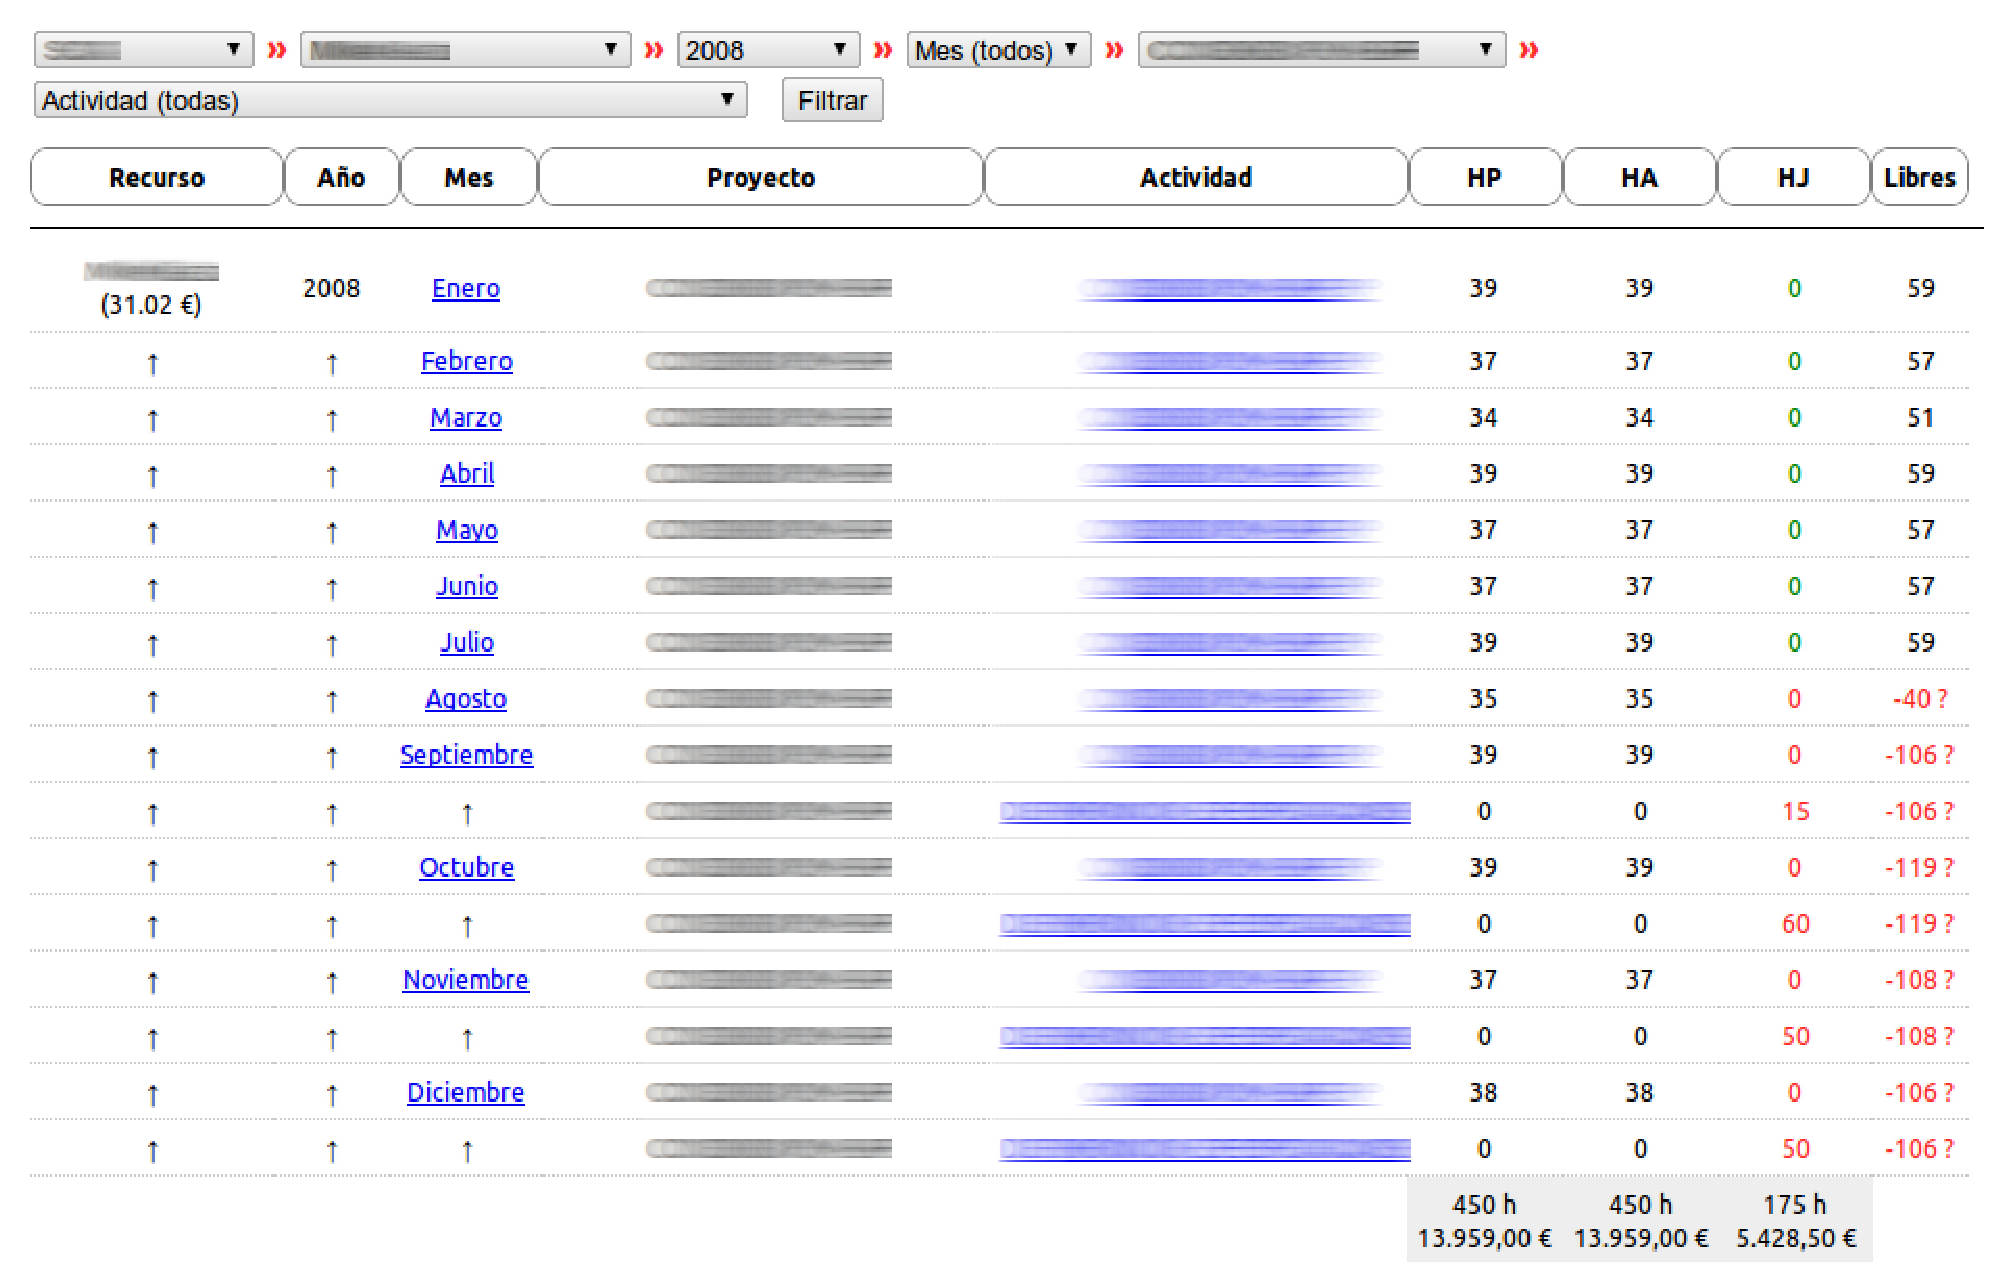
\epsfig{file=imagenes/desglose_mensual.eps,width=5.28in}
% \caption{Vista de desglose mensual por actividades.}
% \label{fig:desglose_mensual}
% \end{figure}

Revisiones muy simples de la distribución de horas del sistema antiguo han
mostrado que en casi la totalidad de los proyectos gestionados se produjo algún
tipo de inconsistencia: a veces dado
por las horas del convenio de los trabajadores y otras, porque a un
recurso se le estaban imputando horas de varios proyectos que
combinadas sobrepasaban el límite mensual supuesto un calendario laboral de 8
horas al día. Con la vista de desglose mensual de la nueva herramienta será muy
fácil filtrar la información para visualizar todas las horas imputadas (en
cualquier proyecto) a un empleado en los meses con inconsistencias.

En el supuesto de una auditoría por parte de los organismos públicos, estas
inconsistencias serían motivo suficiente para que un proyecto subvencionado por
cientos de miles de euros perdiera esa subvención.


\section{Acotación}
\label{sec:acotacion}

Una de las características que definen la aplicación es su respuesta a las
inconsistencias: como se explicó al inicio de la introducción, la herramienta
está pensada para \textit{dejar hacer} y detectar los errores, en lugar de
\textit{no dejar hacer} y proponer soluciones.

\begin{description}
 \item[Caso práctico] Supongamos que queremos grabar en la base de datos la
información del cuadro \ref{tab:distribucion_teorica} acerca de las horas que se
ha proyectado que Pepe Pérez
deberá trabajar en el desarrollo de dos proyectos:

\begin{table}
\centering
\begin{tabular}{|r|c|c||c|}\hline
 & horas proyecto 1  & horas proyecto 2 & total\\\hline\hline
septiembre 2010 & 90 & 110 & 200 \\\hline
octubre 2010 & 90 & 50 & 140\\\hline\hline
total & 180 & 160 & 340\\\hline
\end{tabular}
\caption{Distribución teórica de Pepe Pérez.}
\label{tab:distribucion_teorica}
\end{table}

La inconsistencia se va a dar porque septiembre de 2010 tuvo 22 días laborables,
que se corresponden con 176 horas de trabajo, lejos de las 200 que se están
intentando imputar. Un sistema relativamente avanzado completaría el mes de
septiembre hasta los límites máximos y traspasaría las horas restantes al
siguiente mes, como se muestra en el cuadro \ref{tab:distribucion_ideal}.

\begin{table}
\centering
\begin{tabular}{|r|c|c||c|}\hline
 & horas proyecto 1  & horas proyecto 2 & total \\\hline\hline
septiembre 2010 & 90 & 86 & 176 \\\hline
octubre 2010 & 90 & 74 & 164\\\hline\hline
total & 180 & 160 & 340\\\hline
\end{tabular}
\caption{Distribución ideal de Pepe Pérez.}
\label{tab:distribucion_ideal}
\end{table}

De esta manera, septiembre estaría completo y octubre tendría un total de 164
horas, 4 por debajo del límite mensual marcado por los 21 días laborables que
tuvo ese mes. La inconsistencia habría desaparecido y se habría logrado
conservar el total de horas proyectadas. Sin embargo, esto no siempre va a ser
posible y en el caso que nos ocupa, al tratarse de proyectos de terceros, se
depende de la información que ellos proporcionen y debe grabarse tal cual
llega. Con esta premisa, lo máximo que se puede hacer es informar de la
naturaleza de la inconsistencia para que un técnico busque la solución más
adecuada (véase el cuadro \ref{tab:distribucion_marcada}).

\begin{table}
\centering
\begin{tabular}{|r|c|c||c|}\hline
 & horas proyecto 1  & horas proyecto 2 & total\\\hline\hline
septiembre 2010 & 90 & 110 & {\color{red} 200(-24)} \\\hline
octubre 2010 & 90 & 50 & 140\\\hline\hline
total & 180 & 160 & 340\\\hline
\end{tabular}
\caption{Distribución teórica con marcado de inconsistencias.}
\label{tab:distribucion_marcada}
\end{table}

\end{description}

Hay que recordar que el objetivo de la aplicación se refiere más a la auditoría
de datos y generación de informes que a la de planificación como tal. Esto se
debe, como se ha indicado en el párrafo anterior, a la dependencia de
información externa. La aplicación, sin embargo, sí cuenta con funciones
dedicadas que se emplearán a la hora de planificar proyectos internos de
Ingeniería e Innovación.


